% Options for packages loaded elsewhere
\PassOptionsToPackage{unicode}{hyperref}
\PassOptionsToPackage{hyphens}{url}
\documentclass[
]{book}
\usepackage{xcolor}
\usepackage{amsmath,amssymb}
\setcounter{secnumdepth}{5}
\usepackage{iftex}
\ifPDFTeX
  \usepackage[T1]{fontenc}
  \usepackage[utf8]{inputenc}
  \usepackage{textcomp} % provide euro and other symbols
\else % if luatex or xetex
  \usepackage{unicode-math} % this also loads fontspec
  \defaultfontfeatures{Scale=MatchLowercase}
  \defaultfontfeatures[\rmfamily]{Ligatures=TeX,Scale=1}
\fi
\usepackage{lmodern}
\ifPDFTeX\else
  % xetex/luatex font selection
\fi
% Use upquote if available, for straight quotes in verbatim environments
\IfFileExists{upquote.sty}{\usepackage{upquote}}{}
\IfFileExists{microtype.sty}{% use microtype if available
  \usepackage[]{microtype}
  \UseMicrotypeSet[protrusion]{basicmath} % disable protrusion for tt fonts
}{}
\makeatletter
\@ifundefined{KOMAClassName}{% if non-KOMA class
  \IfFileExists{parskip.sty}{%
    \usepackage{parskip}
  }{% else
    \setlength{\parindent}{0pt}
    \setlength{\parskip}{6pt plus 2pt minus 1pt}}
}{% if KOMA class
  \KOMAoptions{parskip=half}}
\makeatother
\usepackage{color}
\usepackage{fancyvrb}
\newcommand{\VerbBar}{|}
\newcommand{\VERB}{\Verb[commandchars=\\\{\}]}
\DefineVerbatimEnvironment{Highlighting}{Verbatim}{commandchars=\\\{\}}
% Add ',fontsize=\small' for more characters per line
\usepackage{framed}
\definecolor{shadecolor}{RGB}{248,248,248}
\newenvironment{Shaded}{\begin{snugshade}}{\end{snugshade}}
\newcommand{\AlertTok}[1]{\textcolor[rgb]{0.94,0.16,0.16}{#1}}
\newcommand{\AnnotationTok}[1]{\textcolor[rgb]{0.56,0.35,0.01}{\textbf{\textit{#1}}}}
\newcommand{\AttributeTok}[1]{\textcolor[rgb]{0.13,0.29,0.53}{#1}}
\newcommand{\BaseNTok}[1]{\textcolor[rgb]{0.00,0.00,0.81}{#1}}
\newcommand{\BuiltInTok}[1]{#1}
\newcommand{\CharTok}[1]{\textcolor[rgb]{0.31,0.60,0.02}{#1}}
\newcommand{\CommentTok}[1]{\textcolor[rgb]{0.56,0.35,0.01}{\textit{#1}}}
\newcommand{\CommentVarTok}[1]{\textcolor[rgb]{0.56,0.35,0.01}{\textbf{\textit{#1}}}}
\newcommand{\ConstantTok}[1]{\textcolor[rgb]{0.56,0.35,0.01}{#1}}
\newcommand{\ControlFlowTok}[1]{\textcolor[rgb]{0.13,0.29,0.53}{\textbf{#1}}}
\newcommand{\DataTypeTok}[1]{\textcolor[rgb]{0.13,0.29,0.53}{#1}}
\newcommand{\DecValTok}[1]{\textcolor[rgb]{0.00,0.00,0.81}{#1}}
\newcommand{\DocumentationTok}[1]{\textcolor[rgb]{0.56,0.35,0.01}{\textbf{\textit{#1}}}}
\newcommand{\ErrorTok}[1]{\textcolor[rgb]{0.64,0.00,0.00}{\textbf{#1}}}
\newcommand{\ExtensionTok}[1]{#1}
\newcommand{\FloatTok}[1]{\textcolor[rgb]{0.00,0.00,0.81}{#1}}
\newcommand{\FunctionTok}[1]{\textcolor[rgb]{0.13,0.29,0.53}{\textbf{#1}}}
\newcommand{\ImportTok}[1]{#1}
\newcommand{\InformationTok}[1]{\textcolor[rgb]{0.56,0.35,0.01}{\textbf{\textit{#1}}}}
\newcommand{\KeywordTok}[1]{\textcolor[rgb]{0.13,0.29,0.53}{\textbf{#1}}}
\newcommand{\NormalTok}[1]{#1}
\newcommand{\OperatorTok}[1]{\textcolor[rgb]{0.81,0.36,0.00}{\textbf{#1}}}
\newcommand{\OtherTok}[1]{\textcolor[rgb]{0.56,0.35,0.01}{#1}}
\newcommand{\PreprocessorTok}[1]{\textcolor[rgb]{0.56,0.35,0.01}{\textit{#1}}}
\newcommand{\RegionMarkerTok}[1]{#1}
\newcommand{\SpecialCharTok}[1]{\textcolor[rgb]{0.81,0.36,0.00}{\textbf{#1}}}
\newcommand{\SpecialStringTok}[1]{\textcolor[rgb]{0.31,0.60,0.02}{#1}}
\newcommand{\StringTok}[1]{\textcolor[rgb]{0.31,0.60,0.02}{#1}}
\newcommand{\VariableTok}[1]{\textcolor[rgb]{0.00,0.00,0.00}{#1}}
\newcommand{\VerbatimStringTok}[1]{\textcolor[rgb]{0.31,0.60,0.02}{#1}}
\newcommand{\WarningTok}[1]{\textcolor[rgb]{0.56,0.35,0.01}{\textbf{\textit{#1}}}}
\usepackage{longtable,booktabs,array}
\usepackage{calc} % for calculating minipage widths
% Correct order of tables after \paragraph or \subparagraph
\usepackage{etoolbox}
\makeatletter
\patchcmd\longtable{\par}{\if@noskipsec\mbox{}\fi\par}{}{}
\makeatother
% Allow footnotes in longtable head/foot
\IfFileExists{footnotehyper.sty}{\usepackage{footnotehyper}}{\usepackage{footnote}}
\makesavenoteenv{longtable}
\usepackage{graphicx}
\makeatletter
\newsavebox\pandoc@box
\newcommand*\pandocbounded[1]{% scales image to fit in text height/width
  \sbox\pandoc@box{#1}%
  \Gscale@div\@tempa{\textheight}{\dimexpr\ht\pandoc@box+\dp\pandoc@box\relax}%
  \Gscale@div\@tempb{\linewidth}{\wd\pandoc@box}%
  \ifdim\@tempb\p@<\@tempa\p@\let\@tempa\@tempb\fi% select the smaller of both
  \ifdim\@tempa\p@<\p@\scalebox{\@tempa}{\usebox\pandoc@box}%
  \else\usebox{\pandoc@box}%
  \fi%
}
% Set default figure placement to htbp
\def\fps@figure{htbp}
\makeatother
\setlength{\emergencystretch}{3em} % prevent overfull lines
\providecommand{\tightlist}{%
  \setlength{\itemsep}{0pt}\setlength{\parskip}{0pt}}
\usepackage[]{natbib}
\bibliographystyle{apalike}
\usepackage{booktabs}
\usepackage{booktabs}
\usepackage{longtable}
\usepackage{array}
\usepackage{multirow}
\usepackage{wrapfig}
\usepackage{float}
\usepackage{colortbl}
\usepackage{pdflscape}
\usepackage{tabu}
\usepackage{threeparttable}
\usepackage{threeparttablex}
\usepackage[normalem]{ulem}
\usepackage{makecell}
\usepackage{xcolor}
\usepackage{bookmark}
\IfFileExists{xurl.sty}{\usepackage{xurl}}{} % add URL line breaks if available
\urlstyle{same}
\hypersetup{
  pdftitle={Biostatistical method with R code},
  pdfauthor={Shuai Zhu},
  hidelinks,
  pdfcreator={LaTeX via pandoc}}

\title{Biostatistical method with R code}
\author{Shuai Zhu}
\date{2025-07-23}

\begin{document}
\maketitle

{
\setcounter{tocdepth}{1}
\tableofcontents
}
\chapter{前言}\label{ux524dux8a00}

生物统计学方法R代码分享

\chapter{疫苗有效性(Vaccine Efficacy)的样本量计算}\label{ux75abux82d7ux6709ux6548ux6027vaccine-efficacyux7684ux6837ux672cux91cfux8ba1ux7b97}

我们首先导入后面会用到的包,后续会用到dplyr的\%\textgreater\%管道函数和kableExtra输出表格。

\begin{Shaded}
\begin{Highlighting}[]
\FunctionTok{library}\NormalTok{(dplyr)}
\FunctionTok{library}\NormalTok{(kableExtra)}
\end{Highlighting}
\end{Shaded}

\section{疫苗有效性(Vaccine Efficacy)}\label{ux75abux82d7ux6709ux6548ux6027vaccine-efficacy}

\begin{itemize}
\item
  当我们检验一款新的疫苗是否有效时,通常会使用疫苗有效性\(\pi\)(Vaccine Efficacy)这个指标。
\item
  让\(P_1\), \(P_2\)分别为安慰剂组和接种疫苗组的发病率;\(N_1\), \(N_2\)分别为安慰剂组和接种疫苗组的群体总数;\(X, Y\)分别为安慰剂和疫苗组的病例人数。则\(X \overset{i.i.d}{\sim}\text{Binomial}(N_1, P_1)\), \(Y \overset{i.i.d}{\sim}\text{Binomial}(N_2, P_2)\)。
\item
  疫苗有效性可以可以用可以被写成:
  \begin{equation} 
  \pi = 1-(P_2/P_1)
  \label{eq:pi}
  \end{equation}
\item
  原假设和备择假设可以写成
\end{itemize}

\begin{equation} 
  H_0: \pi \leq \pi_0 \text{ versus } \ H_1:\pi>\pi_0   
  \label{eq:hypo1}
\end{equation}

\section{基于泊松假设的大样本}\label{ux57faux4e8eux6ccaux677eux5047ux8bbeux7684ux5927ux6837ux672c}

\begin{itemize}
\item
  如果一个疾病发病率较低,我们就需要更多受试者参加实验,在这种情况下\(X, Y\)可以被近似成为独立的泊松分布.
\item
  \(X \overset{i.i.d}{\sim}\text{Poisson}(\lambda_1)\), \(Y \overset{i.i.d}{\sim}\text{Poisson}(\lambda_2)\) with \(\lambda_1 = N_1\cdot P_1, \lambda_2 = N_2\cdot P_2\).
\item
  \(Y\)的条件概率分布可以被写成
  \(Y|T \sim \text{Binomial}(T, \theta)=\binom{T}{k} \theta^k(1-\theta)^{T-k}\) with \(T = X + Y, \theta = \frac{\lambda_1}{\lambda_1=\lambda_2}\)
\item
  此时原假设和备择假设可以写成
\end{itemize}

\begin{equation} 
  H_0: \theta \geq \theta_0 \text{ versus } \ H_1:\theta<\theta_0 \text{ where } \theta_0 = \frac{1-\pi_0}{2-\pi_0}
  \label{eq:hypo2}
\end{equation}

\begin{itemize}
\item
  P value 可以被计算为
  \begin{equation} 
  p = \Pr[Y \leq Y_{\text{obs}} \mid Y \sim \text{Binomial}(T, \theta_0)] = \sum_{k=0}^{Y_{\text{obs}}} \binom{T}{k} \theta_0^k (1 - \theta_0)^{T - k}
  \label{eq:pvalue}
  \end{equation}
\item
  Statistical power 可以被计算为
  \begin{equation} 
  1 - \beta = \Pr[Y \leq Y_c \mid Y \sim \text{Binomial}(T, \theta_1)] = \sum_{k=0}^{Y_c} \binom{T}{k} \theta_1^k (1 - \theta_1)^{T - k}
  \label{eq:power}
  \end{equation}
\item
  临床实验所需样本量可以被计算为
  \begin{equation} 
  N_2 = T/[(2-\pi_1)/P_1]
  \label{eq:n2}
  \end{equation}
\item
  计算样本量所需的变量为\(\pi_0, \pi_1, \alpha\), 期望统计功效(1-\(\beta\))和安慰剂组发病率(\(P_1\))。
\end{itemize}

\section{R代码示例}\label{rux4ee3ux7801ux793aux4f8b}

\begin{Shaded}
\begin{Highlighting}[]
\NormalTok{exact\_conditonal\_test }\OtherTok{\textless{}{-}} \ControlFlowTok{function}\NormalTok{(T, alpha, power, theta0, theta1) \{}
\NormalTok{  Y\_c }\OtherTok{\textless{}{-}} \FunctionTok{qbinom}\NormalTok{(alpha, }\AttributeTok{size =}\NormalTok{ T, }\AttributeTok{prob =}\NormalTok{ theta0)}\SpecialCharTok{{-}}\DecValTok{1}
\NormalTok{  p\_value }\OtherTok{\textless{}{-}} \FunctionTok{pbinom}\NormalTok{(Y\_c, }\AttributeTok{size =}\NormalTok{ T, }\AttributeTok{prob =}\NormalTok{ theta0)}
\NormalTok{  power }\OtherTok{\textless{}{-}} \FunctionTok{pbinom}\NormalTok{(Y\_c, }\AttributeTok{size =}\NormalTok{ T, }\AttributeTok{prob =}\NormalTok{ theta1)}
  \FunctionTok{return}\NormalTok{(}\FunctionTok{c}\NormalTok{(T, Y\_c, power, p\_value))}
\NormalTok{\}}

\NormalTok{ect\_sample\_size }\OtherTok{\textless{}{-}} \ControlFlowTok{function}\NormalTok{(T, pi0, pi1, incidence, alpha, power)\{}
\NormalTok{  theta0 }\OtherTok{\textless{}{-}}\NormalTok{ (}\DecValTok{1}\SpecialCharTok{{-}}\NormalTok{pi0) }\SpecialCharTok{/}\NormalTok{ (}\DecValTok{2}\SpecialCharTok{{-}}\NormalTok{pi0)}
\NormalTok{  theta1 }\OtherTok{\textless{}{-}}\NormalTok{ (}\DecValTok{1}\SpecialCharTok{{-}}\NormalTok{pi1) }\SpecialCharTok{/}\NormalTok{ (}\DecValTok{2}\SpecialCharTok{{-}}\NormalTok{pi1)}
\NormalTok{  table\_t }\OtherTok{\textless{}{-}} \FunctionTok{as.data.frame}\NormalTok{(}\FunctionTok{do.call}\NormalTok{(rbind, }
                               \FunctionTok{lapply}\NormalTok{(T, exact\_conditonal\_test, }\AttributeTok{alpha =}\NormalTok{ alpha, }\AttributeTok{theta0=}\NormalTok{ theta0, }\AttributeTok{theta1 =}\NormalTok{ theta1)), }\AttributeTok{.name\_repair =} \StringTok{"unique"}\NormalTok{)}
  \FunctionTok{colnames}\NormalTok{(table\_t) }\OtherTok{\textless{}{-}} \FunctionTok{c}\NormalTok{(}\StringTok{\textquotesingle{}T\textquotesingle{}}\NormalTok{, }\StringTok{\textquotesingle{}Y\_c\textquotesingle{}}\NormalTok{, }\StringTok{\textquotesingle{}power\textquotesingle{}}\NormalTok{, }\StringTok{\textquotesingle{}p{-}value\textquotesingle{}}\NormalTok{)}
  
  \ControlFlowTok{for}\NormalTok{ (n }\ControlFlowTok{in} \DecValTok{1}\SpecialCharTok{:}\FunctionTok{nrow}\NormalTok{(table\_t))\{}
    \ControlFlowTok{if}\NormalTok{ (table\_t}\SpecialCharTok{$}\NormalTok{power[n] }\SpecialCharTok{\textgreater{}=}\NormalTok{ power }\SpecialCharTok{\&\&} \FunctionTok{all}\NormalTok{(table\_t}\SpecialCharTok{$}\NormalTok{power[n}\SpecialCharTok{:}\FunctionTok{nrow}\NormalTok{(table\_t)] }\SpecialCharTok{\textgreater{}=}\NormalTok{ power)) \{}
\NormalTok{      min\_n }\OtherTok{\textless{}{-}}\NormalTok{ table\_t}\SpecialCharTok{$}\NormalTok{T[n]}
      \ControlFlowTok{break}
\NormalTok{    \}}
\NormalTok{  \}}
\NormalTok{  result }\OtherTok{\textless{}{-}} \FunctionTok{list}\NormalTok{(}
    \AttributeTok{T\_table =}\NormalTok{ table\_t,}
    \AttributeTok{T =}\NormalTok{ min\_n,}
    \AttributeTok{text =} \FunctionTok{paste0}\NormalTok{(}\StringTok{\textquotesingle{}The min value of T achieve power of \textquotesingle{}}\NormalTok{, power, }\StringTok{\textquotesingle{} is \textquotesingle{}}\NormalTok{, min\_n)}
\NormalTok{  )}
  \FunctionTok{class}\NormalTok{(result) }\OtherTok{\textless{}{-}} \StringTok{\textquotesingle{}result\textquotesingle{}}
\NormalTok{  result}
\NormalTok{\}}

\NormalTok{print.myresult }\OtherTok{\textless{}{-}} \ControlFlowTok{function}\NormalTok{(x, ...) \{}
  \FunctionTok{cat}\NormalTok{(x}\SpecialCharTok{$}\NormalTok{text, }\StringTok{"}\SpecialCharTok{\textbackslash{}n}\StringTok{"}\NormalTok{)}
\NormalTok{\}}


\NormalTok{T2N }\OtherTok{\textless{}{-}} \ControlFlowTok{function}\NormalTok{(T\_value, incidence, pi1, dropout\_rate)\{}
\NormalTok{  N2 }\OtherTok{\textless{}{-}}\NormalTok{ T\_value}\SpecialCharTok{/}\NormalTok{((}\DecValTok{2}\SpecialCharTok{{-}}\NormalTok{pi1)}\SpecialCharTok{*}\NormalTok{incidence)}\SpecialCharTok{/}\NormalTok{(}\DecValTok{1}\SpecialCharTok{{-}}\NormalTok{dropout\_rate)}
  \FunctionTok{cat}\NormalTok{(}\StringTok{\textquotesingle{}The sample of vaccine group considering the drop out rate:\textquotesingle{}}\NormalTok{, N2)}
\NormalTok{\}}
\end{Highlighting}
\end{Shaded}

详细推导过程可以看 \citet{chan_exact_1998} 和 \citet{loiacono_sample_nodate}

\subsection{例1}\label{ux4f8b1}

\citet{chan_exact_1998} 这篇论文介绍了exact conditional method的公式推导。他还给了一个不同样本量对应的power和significance level。 我们可以运行上面的函数来验证结果的准确性。设置病例范围从33到40,\(\pi_0=0.2,\pi_1=0.8, P_1=0.006, \alpha=0.025\), 期望统计功效为95\%。输入以上参数到ect\_sample\_size这个函数。

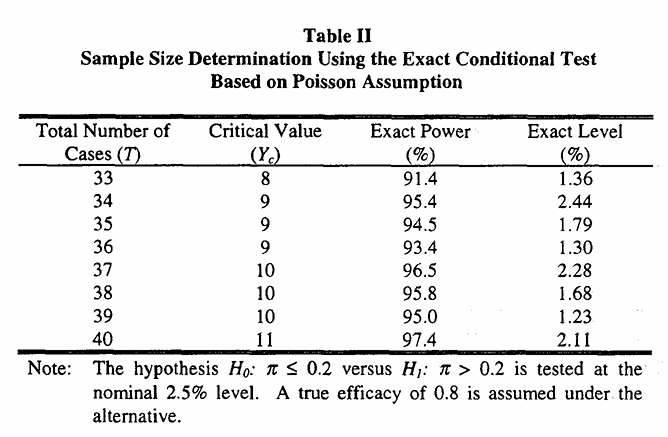
\includegraphics[width=9.28in]{image/Screenshot 2025-07-21 155606}

\begin{Shaded}
\begin{Highlighting}[]
\NormalTok{T }\OtherTok{\textless{}{-}} \DecValTok{33}\SpecialCharTok{:}\DecValTok{40} \CommentTok{\# the number of T}
\NormalTok{pi0 }\OtherTok{\textless{}{-}} \FloatTok{0.2} \CommentTok{\# null hypothesis efficacy}
\NormalTok{pi1 }\OtherTok{\textless{}{-}} \FloatTok{0.8} \CommentTok{\# True efficacy under alternative hypothesis}
\NormalTok{alpha }\OtherTok{\textless{}{-}} \FloatTok{0.025} \CommentTok{\# type I error}
\NormalTok{incidence }\OtherTok{\textless{}{-}} \FloatTok{0.006} \CommentTok{\# placebo incidence rate}
\NormalTok{power }\OtherTok{\textless{}{-}} \FloatTok{0.95}
\NormalTok{res1 }\OtherTok{\textless{}{-}} \FunctionTok{ect\_sample\_size}\NormalTok{(T, pi0, pi1, incidence, alpha, power)}
\FunctionTok{kbl}\NormalTok{(res1}\SpecialCharTok{$}\NormalTok{T\_table)}\SpecialCharTok{\%\textgreater{}\%} 
  \FunctionTok{kable\_styling}\NormalTok{(}\AttributeTok{bootstrap\_options =} \StringTok{"striped"}\NormalTok{, }\AttributeTok{full\_width =}\NormalTok{ F, }\AttributeTok{position =} \StringTok{"left"}\NormalTok{)}
\end{Highlighting}
\end{Shaded}

\begin{tabular}[t]{r|r|r|r}
\hline
T & Y\_c & power & p-value\\
\hline
33 & 8 & 0.9139690 & 0.0136117\\
\hline
34 & 9 & 0.9540856 & 0.0244451\\
\hline
35 & 9 & 0.9449925 & 0.0178969\\
\hline
36 & 9 & 0.9347919 & 0.0129998\\
\hline
37 & 10 & 0.9653937 & 0.0227940\\
\hline
38 & 10 & 0.9584044 & 0.0168288\\
\hline
39 & 10 & 0.9504998 & 0.0123313\\
\hline
40 & 11 & 0.9738542 & 0.0211901\\
\hline
\end{tabular}

代码中的incidence 就是\(P_1\), 其他参数与上面提及的保持一致。可以看到输出的表格中样本量,critical value, statistical power和p value与论文中的表格完全一致。我们打印出能够达到95\% statistical power的病例数

\begin{Shaded}
\begin{Highlighting}[]
\NormalTok{res1}\SpecialCharTok{$}\NormalTok{T}
\CommentTok{\#\textgreater{} [1] 37}
\end{Highlighting}
\end{Shaded}

打印出T=37与论文一致,再用公式\eqref{eq:n2}计算出疫苗组样本量,为了方便计算我也写成了函数t2n。此示例计算样本量时没有考虑脱落所以dropout\_rate 参数可以设置为0。得到结果样本量至少为5138.889。这个结果乘2就是疫苗组和安慰剂组所需的总样本量,总样本量至少为10277.78,进一10278。此结果与论文一致,证明我们的算法无误。

\begin{Shaded}
\begin{Highlighting}[]
\FunctionTok{T2N}\NormalTok{(}\DecValTok{37}\NormalTok{, incidence, pi1, }\AttributeTok{dropout\_rate =} \DecValTok{0}\NormalTok{)}
\CommentTok{\#\textgreater{} The sample of vaccine group considering the drop out rate: 5138.889}
\end{Highlighting}
\end{Shaded}

\subsection{HRV-三期}\label{hrv-ux4e09ux671f}

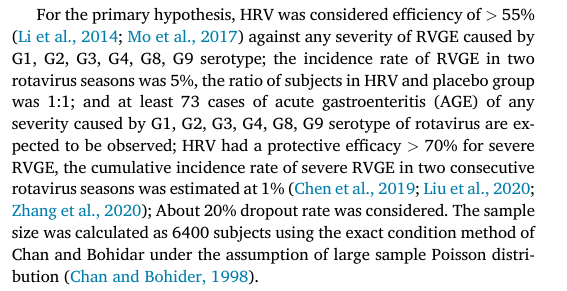
\includegraphics[width=7.88in]{image/Screenshot 2025-07-22 173413}

\citet{wu_efficacy_2022} 这篇论文原为我们想要复现的样本量。但是过程中发现其中并未明确提及所需参数 \(\pi_1, \alpha\)和期望统计功效。无法计算出样本量所以后续我们使用这篇论文作为参考。下一个示例为HRV-三期这篇论文的参考文献,也是rotavirus vaccine的疫苗有效性临床实验。

\subsection{RV5}\label{rv5}

\citet{mo_efficacy_2017} 这篇论文会作为我们后续疫苗有效性检验样本量计算的参考文章。提供参数:15\%脱落率, \(\pi_0=0, \pi_1=0.6, P_1 = 0.02, \alpha = 0.025\),期望统计功效为80\%。带入以上参数可以得到病例总数至少为47,我们取双数48。再用T2N函数计算疫苗组样本量总数至少2016.807,我们取整为2020,与论文一致。

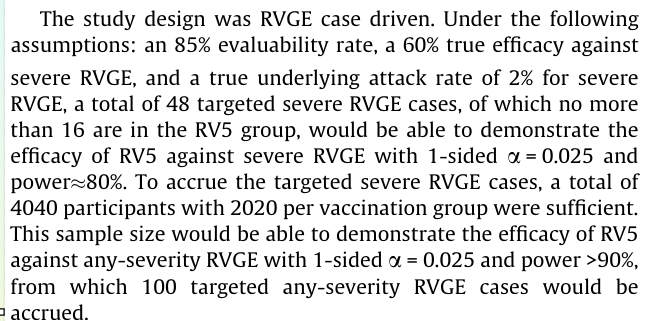
\includegraphics[width=9.11in]{image/Screenshot 2025-07-21 162616}

\begin{Shaded}
\begin{Highlighting}[]
\NormalTok{T }\OtherTok{\textless{}{-}} \DecValTok{40}\SpecialCharTok{:}\DecValTok{50} \CommentTok{\# the number of T}
\NormalTok{pi0 }\OtherTok{\textless{}{-}} \DecValTok{0} \CommentTok{\# null hypothesis efficacy}
\NormalTok{pi1 }\OtherTok{\textless{}{-}} \FloatTok{0.6} \CommentTok{\# True efficacy under alternative hypothesis}
\NormalTok{alpha }\OtherTok{\textless{}{-}} \FloatTok{0.025} \CommentTok{\# type I error}
\NormalTok{incidence }\OtherTok{\textless{}{-}} \FloatTok{0.02} \CommentTok{\# placebo incidence rate}
\NormalTok{power }\OtherTok{\textless{}{-}} \FloatTok{0.8}
\NormalTok{res\_rv5 }\OtherTok{\textless{}{-}} \FunctionTok{ect\_sample\_size}\NormalTok{(T, pi0, pi1, incidence, alpha, power)}
\FunctionTok{kbl}\NormalTok{(res\_rv5}\SpecialCharTok{$}\NormalTok{T\_table)}\SpecialCharTok{\%\textgreater{}\%} 
  \FunctionTok{kable\_styling}\NormalTok{(}\AttributeTok{bootstrap\_options =} \StringTok{"striped"}\NormalTok{, }\AttributeTok{full\_width =}\NormalTok{ F, }\AttributeTok{position =} \StringTok{"left"}\NormalTok{)}
\end{Highlighting}
\end{Shaded}

\begin{tabular}[t]{r|r|r|r}
\hline
T & Y\_c & power & p-value\\
\hline
40 & 13 & 0.7692914 & 0.0192387\\
\hline
41 & 13 & 0.7363326 & 0.0137666\\
\hline
42 & 14 & 0.8052771 & 0.0217793\\
\hline
43 & 14 & 0.7757295 & 0.0157697\\
\hline
44 & 15 & 0.8362319 & 0.0243834\\
\hline
45 & 15 & 0.8100042 & 0.0178489\\
\hline
46 & 15 & 0.7819032 & 0.0129480\\
\hline
47 & 16 & 0.8396107 & 0.0199930\\
\hline
48 & 16 & 0.8146130 & 0.0146525\\
\hline
49 & 17 & 0.8650285 & 0.0221921\\
\hline
50 & 17 & 0.8429717 & 0.0164196\\
\hline
\end{tabular}

\begin{Shaded}
\begin{Highlighting}[]
\NormalTok{res\_rv5}\SpecialCharTok{$}\NormalTok{T}
\CommentTok{\#\textgreater{} [1] 47}
\end{Highlighting}
\end{Shaded}

\begin{Shaded}
\begin{Highlighting}[]
\FunctionTok{T2N}\NormalTok{(}\DecValTok{48}\NormalTok{, incidence, pi1, }\AttributeTok{dropout\_rate =} \FloatTok{0.15}\NormalTok{)}
\CommentTok{\#\textgreater{} The sample of vaccine group considering the drop out rate: 2016.807}
\end{Highlighting}
\end{Shaded}

\section*{Reference}\label{reference}
\addcontentsline{toc}{section}{Reference}

\bibliography{reference.bib}

\end{document}
